\documentclass[12pt, letterpaper, titlepage]{article}

\usepackage{amsmath}
\usepackage{booktabs}
\usepackage{amsthm}
\usepackage{graphicx}
\usepackage[margin=1in]{geometry}
\usepackage{hyperref}
\hypersetup{colorlinks = true, linkcolor = blue, citecolor=blue, urlcolor = blue}
\usepackage{natbib}
\usepackage{enumitem}
\usepackage{setspace}

\usepackage[pagewise]{lineno}
\linenumbers*[1]
% %% patches to make lineno work better with amsmath
\newcommand*\patchAmsMathEnvironmentForLineno[1]{%
 \expandafter\let\csname old#1\expandafter\endcsname\csname #1\endcsname
 \expandafter\let\csname oldend#1\expandafter\endcsname\csname end#1\endcsname
 \renewenvironment{#1}%
 {\linenomath\csname old#1\endcsname}%
 {\csname oldend#1\endcsname\endlinenomath}}%
\newcommand*\patchBothAmsMathEnvironmentsForLineno[1]{%
 \patchAmsMathEnvironmentForLineno{#1}%
 \patchAmsMathEnvironmentForLineno{#1*}}%

\AtBeginDocument{%
 \patchBothAmsMathEnvironmentsForLineno{equation}%
 \patchBothAmsMathEnvironmentsForLineno{align}%
 \patchBothAmsMathEnvironmentsForLineno{flalign}%
 \patchBothAmsMathEnvironmentsForLineno{alignat}%
 \patchBothAmsMathEnvironmentsForLineno{gather}%
 \patchBothAmsMathEnvironmentsForLineno{multline}%
}

\makeatletter
\newcommand*{\Xbar}{}%
\DeclareRobustCommand*{\Xbar}{%
  \mathpalette\@Xbar{}%
}
\newcommand*{\@Xbar}[2]{%
  % #1: math style
  % #2: unused (empty)
  \sbox0{$#1\mathrm{X}\m@th$}%
  \sbox2{$#1X\m@th$}%
  \rlap{%
    \hbox to\wd2{%
      \hfill
      $\overline{%
        \vrule width 0pt height\ht0 %
        \kern\wd0 %
      }$%
    }%
  }%
  \copy2 %
}
\makeatother

\title{Survey of Misuses of the Kolmogorov–Smirnov-Test}

\author{Anthony Zeimbekakis and Jun Yan\\
\href{mailto:anthony.zeimbekakis@uconn.edu}{\nolinkurl{anthony.zeimbekakis@uconn.edu}}\\
Department of Statistics, University of Connecticut}
\date{January 23, 2021}

\begin{document}
\maketitle

\doublespace

\begin{abstract}
The Kolmogorov-Smirnov (KS) test is one the most popular goodness-of-fit tests for comparing a sample with a hypothesized parametric distribution. Nevertheless, it has often been misused. The standard one-sample KS test applies to independent, continuous data with a hypothesized distribution that is completely specified. It is not uncommon, however, to see in the literature that it was applied to dependent, discrete, or rounded data, with hypothesized distributions containing estimated parameters. For example, it has been “discovered” multiple times that the test is too conservative when the parameters are estimated [e.g. \citet{Steinskog}]. This paper aims to survey the misuses of the KS test, demonstrate their consequences through simulation, and provide remedies as needed.
\end{abstract}


\hypertarget{sec:intro}{%
\section{Introduction}\label{sec:intro}}

The Kolmogorov-Smirnov (K-S) statistic is one of the most popular goodness-of-fit tests for comparing a sample with a hypothesized parametric distribution. Given a sample of n observations, let $S_{n}(x)$ be the empirical cumulative distribution and $F(x)$ be the population cumulative distribution. The K-S statistic is defined by: \[d = max(\lvert F(x)-S_{n}(x) \rvert)\] The null hypothesis is that the observations are from the specified distribution $F(x)$, and the alternate hypothesis is that the data is not from $F(x)$. If the value of $d$ exceeds the critical value given by a table, the null hypothesis is rejected.

However, the test is often misused. The standard one-sample K-S test applies to independent, continuous data with a hypothesized distribution that is completely specified. Often in literature, the test is applied to dependent, discrete, or rounded data, with hypothesized distributions containing estimated parameters. As shown by \citet{Steinskog} and later in this paper, the test is too conservative when the parameters are estimated. Throughout this paper, the cumulative distribution $F(x)$ is standard normal.

\hypertarget{sec:fitted}{%
\section{Fitted Parameters}\label{sec:fitted}}

The K-S test shows significant issues in the case of fitted parameters. As previously mentioned, one assumption of the K-S test is that the hypothesized distribution is completely specified. However, the procedure is sometimes performed where the population cumulative distribution $F(x)$ has parameters $\mu=\Xbar$, the sample mean, and $\sigma^2=s^2$, the sample variance \citep{Lilliefors}. \citet{Lilliefors} also shows that using the standard table when values of the mean and standard deviation are estimated obtains extremely conservative results. 

To resolve this problem, parametric bootstrap can be performed. The parameters of the null distribution are approximated from the bootstrap. Figure~\ref{fig:hist_parametric} displays the results of $1000$ replicate tests using the standard normal distribution with sample size $n=100$. In each parametric test, $1000$ bootstrap samples are obtained and the corresponding p-value of the K-S test is calculated. In the naive case, K-S tests are performed with fitted parameters.

\begin{figure}[tbp]
  \centering
  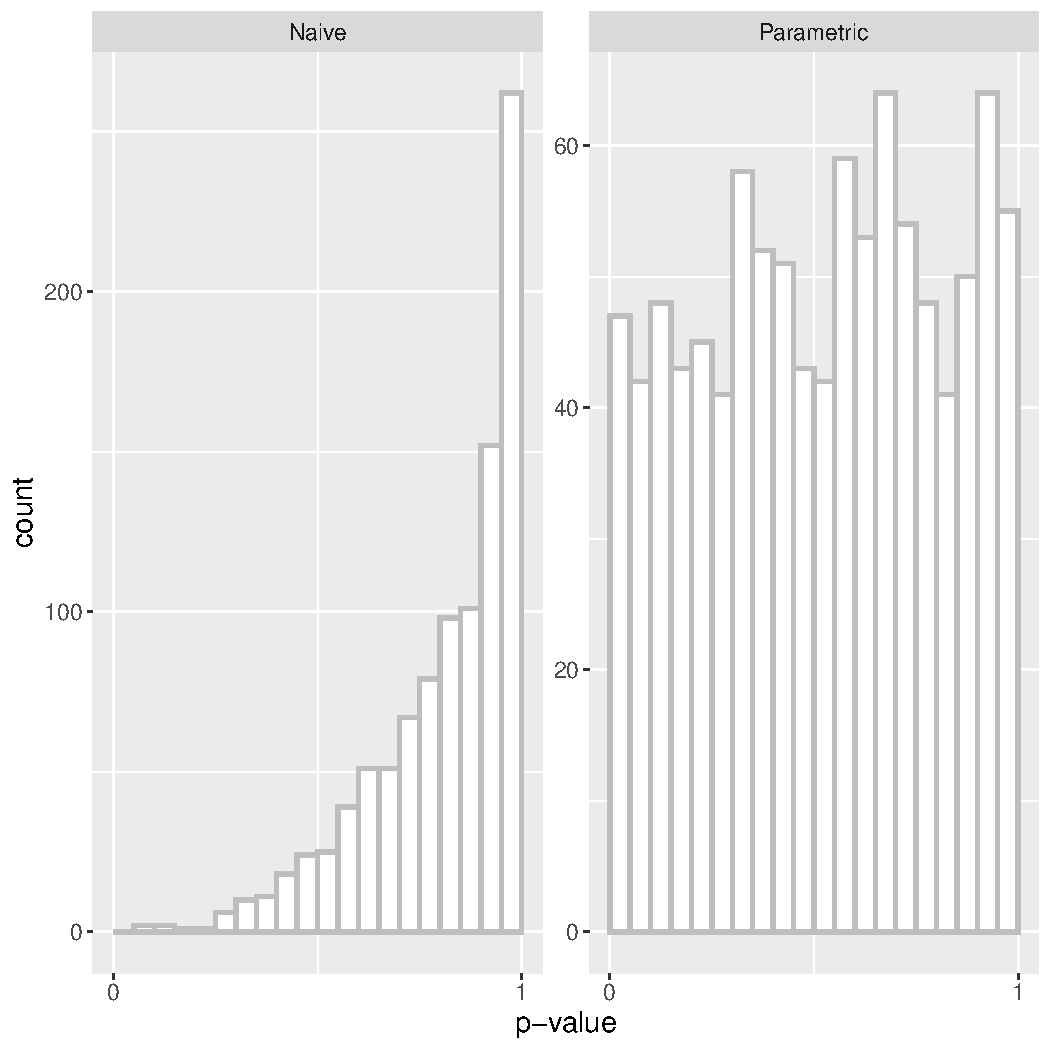
\includegraphics{hist_parametric}
  \caption{Histograms demonstrating fitted parameters.}
  \label{fig:hist_parametric}
\end{figure}

Since the data is generated from a standard normal distributions with seemingly all assumptions met, a uniform distribution of $U(0,1)$ is expected for the p-values. The naive histogram shows that when the parameters are estimated there is notable deviation from the uniform distribution. However, through parametric bootstrap of the parameters the p-values appear to retain a uniform distribution.

\hypertarget{sec:rounded}{%
\section{Rounded Data}\label{sec:rounded}}

Another assumption of the K-S test is that it applies to continuous data. This can be easily violated by performing a level of rounding on the data. Rounding causes the data to become discrete, and the K-S test can be shown to no longer apply. To demonstrate this, simulations were conducted at varying levels of rounding. A random sample of size $100$ was collected from the standard normal distribution and subsequently rounded to the degrees of $.01$ and  $.1$. This simulation was replicated $1000$ times for each rounding level and the results are shown in Figure~\ref{fig:hist_rounded}.

\begin{figure}[tbp]
  \centering
  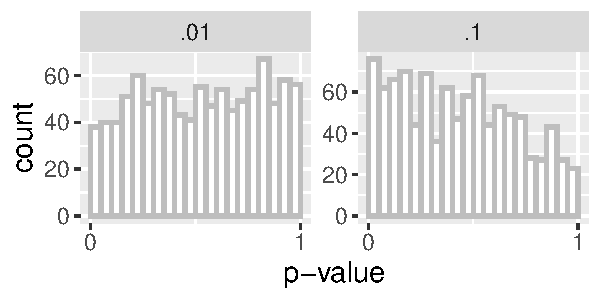
\includegraphics{hist_rounded}
  \caption{Histograms of P-values with rounded data.}
  \label{fig:hist_rounded}
\end{figure}

As mentioned before, the expected distribution of p-values is $U(0,1)$. For rounding to the hundreths, though the distribution appears uniform it is still not recommended to use the basic K-S test due to ties in the data. The issue is apparent when rounding to the tenths, as the distribution of p-values does not hold a standard uniform distribution and the test no longer applies. This simulation shows that rounding can have a serious impact on the power of the K-S test and should be avoided.

There are some solutions in the case that a discrete distribution is in question. The chi-squared test is another goodness-of-fit test that can be applied to discrete distributions \citep{Massey}. However, the standard K-S test holds various advantages over it. In small samples, \citet{Massey} explains that the chi-squared test loses information and validity due to the grouping performed, while the K-S test treats individual observations separately. \citet{Massey} additionally notes that the K-S test generally appears to be the more powerful test regardless of sample size.

In addition, a proposed revision of the K-S test can be found in \citet{dgof}.\citet{dgof} provides a revision to R's `ks.test()` function for the case that the null distribution is discrete.

\begin{figure}[tbp]
  \centering
  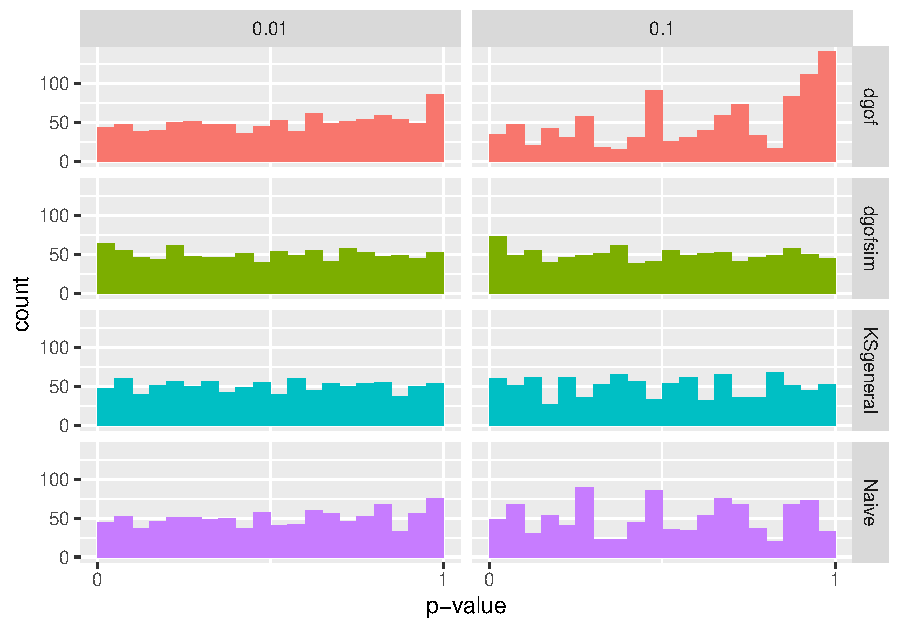
\includegraphics{hist_general}
  \caption{Histograms of P-values with KSGeneral and dgof packages.}
  \label{fig:hist_general}
\end{figure}

\hypertarget{sec:correlation}{%
\section{Problem under Serial Dependence}\label{sec:correlation}}

The K-S test shows significant issues in the case of serial dependence.

\begin{figure}[tbp]
  \centering
  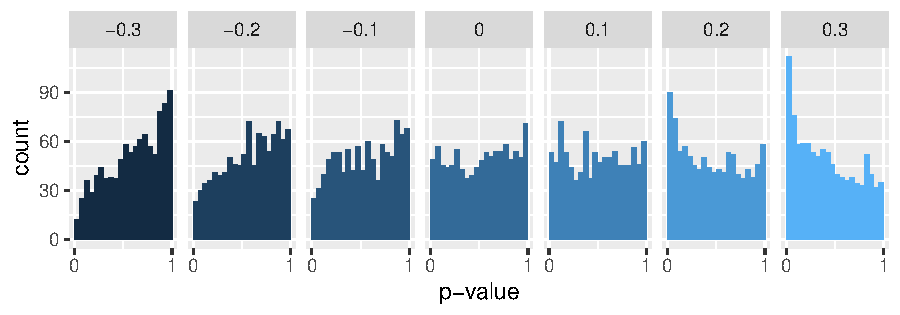
\includegraphics{hist_correlation}
  \caption{Histograms of P-values with correlated data.}
  \label{fig:hist_correlation}
\end{figure}

\begin{figure}[tbp]
  \centering
  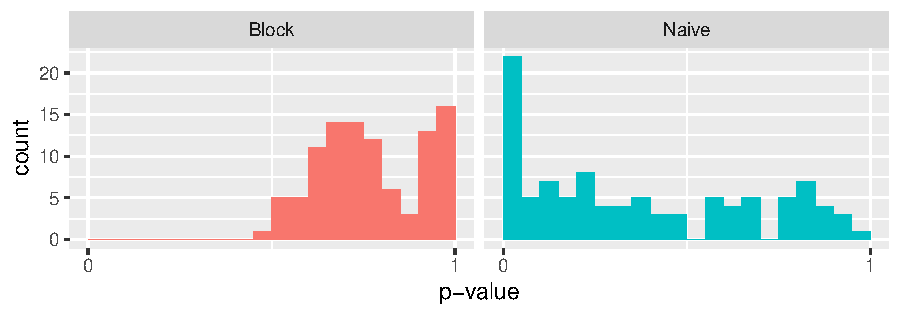
\includegraphics{hist_block}
  \caption{Histograms of P-values when using block bootstrap.}
  \label{fig:hist_block}
\end{figure}

\hypertarget{sec:conclusion}{%
\section{Conclusion}\label{sec:conclusion}}

Conclusion here.

Adding these to see the full bibliography: 

\citet{Steinskog}
\citet{Weiss}
\citet{Massey}
\citet{Lilliefors}
\citet{Arnold}
\citet{Conover}
\citet{Gleser}
\citet{Babu}
\citet{Butorina}
\citet{Racine}
\citet{Wang}
\citet{Capasso}
\citet{Dimitrova}

\bibliographystyle{chicago}
\bibliography{citations.bib}


\end{document}
